\documentclass[12pt]{article} 
\usepackage{graphicx} 
\usepackage{amsmath}
\usepackage{natbib}
\bibliographystyle{plain}
% Increase margins (manually) 
  % Sides (odd- and even-numbered pages)
    \addtolength{\oddsidemargin}{-0.875in}
    \addtolength{\evensidemargin}{-0.875in}
    \addtolength{\textwidth}{1.75in}
  % Top/bottom
    \addtolength{\topmargin}{-0.875in}
    \addtolength{\textheight}{1.75in}
\title{ASTR 565 \\
Computer Problem 2.1: Polytropes}
\author{Laurel Farris}
\date{06 October 2015}
\begin{document}
\maketitle
\section{Introduction}
Polytropes are gaseous spheres in hydrostatic equilibrium whose
pressure and density at any point along the radius are related by:
\begin{equation}
P = K\rho^{(n+1)/n}
\end{equation}
where $K$ is a constant and $n$ is the polytropic index.
The structure of a polytrope can be modeled using the \emph{Lane-Emden
equation}:
\begin{equation}
  \frac{1}{\xi^2}\frac{d}{d\xi}\left(\xi^2\frac{d\theta}{d\xi}\right) =
  -{\theta^n}
\end{equation}
where $\xi$ is a dimensionless quantity that represents distance from
the center of the sphere. This
relationship is a simplification following from the combination of hydrostatic
equilibrium and equation (1). \cite{clayton}

\section{Methods}
Exact solutions only exist for $n$
= 0, 1, and 5, so solutions for other values must be approximated
using numerical techniques. Since the \emph{Lane-Emden
equation} is a second-order differential equation, the best approach
was to first express it as two first-order differential equations. Replacing
$\xi$ with $x$ and $\theta$ with $y$, we have: 
\begin{equation}
 y' = z
\end{equation}
and
\begin{equation}
 z' = -\left(\frac{2}{x}\right)z -y^n
\end{equation}
where $z$ is a new variable equal to $dy/dx$.

To approximate $y$ ($\theta$) as a function of $x$ ($\xi$), the \emph{Runge-Kutta}
method\cite{recipes} was used to the fourth-order. Given boundary conditions at the
center: $x_o = 0$ and $y_o = 1$, and at the surface: $y_1 = 0$, $y$
was approximated by stepping from the center(0) to the surface(1)
using the following equations:
\begin{align*}
k_1 &= hf(x_n,y_n)\\
k_2 &= hf(x_n+\frac{1}{2}h,y_n+\frac{1}{2}k_1)\\
k_3 &= hf(x_n+\frac{1}{2}h,y_n+\frac{1}{2}k_2)\\
k_4 &= hf(x_n+h,y_n+k_3)\\
y_{n+1} &=
y_n+\frac{1}{6}k_1+\frac{1}{3}k_2+\frac{1}{3}k_3+\frac{1}{6}k_4+O(h^5)\\
\end{align*}
 The first four correspond to the ``fourth order" part of the
approximation and were calculated for every step $h$ through $x$ to
generate the next value for $y$ (with the exception 
of $O(h^5)$ in the last equation, which is 
a margin of error that was not included here).
This process was
repeated until $y$ reached the surface boundary condition.
Similar equations were used to approximate
$z$ ($dy/dx$), replacing $k$ with $l$.

\section{Results}
Returning to the original symbols, the values for $\xi_1$ ($\xi$ at
the surface) and
other parameters for a polytropic index of $n$ = 4.5 are listed in
table \ref{table:nonlin}. 

\begin{table}[h]
\caption{Values for polytropic index $n$ = 4.5}
\centering
\begin{tabular}{ c c c c c c c c c  }
 \hline\hline
$n$ & $\xi_1$ & $\rho_c/\rho$ & $N_{n}$ & $W_n$ & $\Theta_n$ 
& $\rho_c[g\,cm^{-3}]$ & $P_c[dyne\,cm^{-2}]$ & $T_c[K]$ \\
\hline
4.5 & 31.841 & 6187.500 & 0.658 & 4917.415 & 3.329 & 8718.704 &
5.535e19 & 4.742e7 \\
\hline
\end{tabular}\\
\label{table:nonlin}
\end{table}

The resulting approximation for $\theta$ is plotted in figure
\ref{plot}, along with $\theta^n$, $\theta^{n+1}$, and $q$.
\begin{figure}[h]
\centering
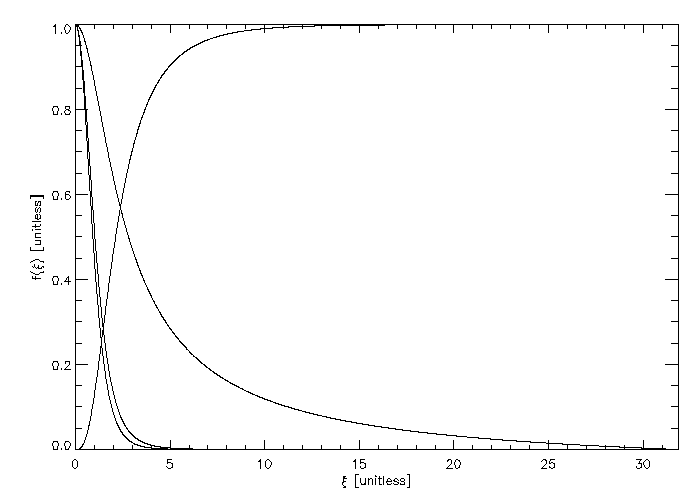
\includegraphics[width=7.0in]{plot2.png}
\caption{This plot shows $\theta$ (red), 
$\theta^n$ (green),
$\theta^{n+1}$ (blue),
and $q$ (purple) 
as functions of $\xi$.} 
\label{plot}
\end{figure}
$\theta^n$ = $\rho/\rho_c$, where $\rho_c$ is the density at the center 
of the star. Therefore, $\theta^n$ for any value of n is always equal
to $1$ at the center, and $0$ at the surface, where the density is assumed
 to fall to $0$, as shown in figure \ref{plot}. This was how the boundary 
 conditions were determined for the \emph{Runge-Kutta} method. The mass 
 distribution is represented by $q$, which can be expressed as:
\begin{equation}
 q = \frac{m}{M} = \left(\xi^2\frac{d\theta}{d\xi}\right)
                   \left(\xi^{2}_{1}\frac{d\theta}{d\xi_1}\right)^{-1}
\end{equation}
and increases from $0$ to $1$ in figure \ref{plot}.

\newpage
\bibliography{reffile}
\end{document}


